\documentclass[12pt]{article}


\usepackage[margin=1.1in,footskip=.25in]{geometry}

\usepackage{tabularx}
\usepackage[table]{xcolor}
\usepackage{multirow}

\newcolumntype{C}{ >{\centering\arraybackslash} m{5cm} }
\newcolumntype{E}{ >{\centering\arraybackslash} m{7cm} }
\newcolumntype{D}{ >{\centering\arraybackslash} m{3cm} }
\newcolumntype{F}{ >{\centering\arraybackslash} m{1cm} }
\newcolumntype{G}{ >{\centering\arraybackslash} m{2cm} }

\usepackage{array}

\usepackage{tikz} 
\usetikzlibrary{graphs,quotes,arrows.meta}
\usetikzlibrary{automata}
\usetikzlibrary{positioning}
\usetikzlibrary{patterns}
\usetikzlibrary{matrix,backgrounds}
\usetikzlibrary{arrows,shapes,trees}
\usetikzlibrary{chains}
\usetikzlibrary{calc}


\tikzstyle{vertex}=[draw,fill=black!5,circle,minimum size=20pt,inner sep=1pt]
\tikzstyle{error}=[fill=red!60]

\tikzset{
  treenode/.style = {align=center, inner sep=0pt, text centered,
    font=\sffamily},
  arn_n/.style = {treenode, circle, white, font=\sffamily\bfseries, draw=black,
    fill=black, text width=1.5em},% arbre rouge noir, noeud noir
  arn_r/.style = {treenode, circle, red, draw=red, 
    text width=1.5em, very thick},% arbre rouge noir, noeud rouge
  arn_x/.style = {treenode, rectangle, draw=black,
    minimum width=0.5em, minimum height=0.5em}% arbre rouge noir, nil
}

\usepackage{amsmath, amssymb}
\usepackage{mathtools}
\makeatletter
\def\env@cases{%
  \let\@ifnextchar\new@ifnextchar
  \left\lbrace
  \def\arraystretch{1.2}%
  \array{l@{\quad}l@{}}% Formerly @{}l@{\quad}l@{}
}
\makeatother



\usepackage[most]{tcolorbox}

\tcbset{
    frame code={}
    center title,
    left=10pt,
    right=10pt,
    top=10pt,
    bottom=10pt,
    colback=gray!5,
    colframe=gray,
    width=\dimexpr\textwidth\relax,
    enlarge left by=0mm,
    boxsep=5pt,
    arc=0pt,outer arc=0pt,
}

\renewcommand{\baselinestretch}{1.3} 

\begin{document}

\tableofcontents

\newpage

\section{Introduction to AVL Trees}

\begin{enumerate}
	\item what is a Binary Search Tree (BST)
	\item Drawback of BST
	\item How BST can be improved
	\item what is an AVL Tree
	\item Rotation in AVL Tree
	\item How to create AVL Tree
\end{enumerate}


\section{Binary Search Tree}

\begin{center}
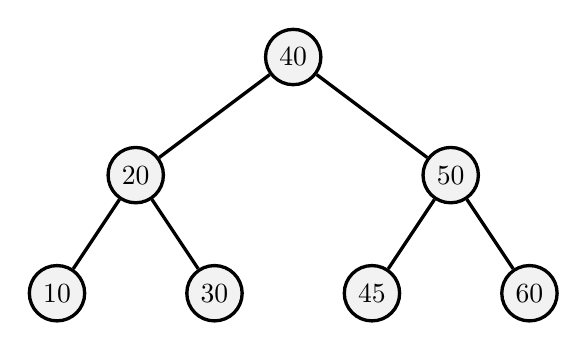
\begin{tikzpicture}[very thick,level/.style={sibling distance=40mm/#1}]
\tikzstyle{vertex}=[draw,fill=black!5,circle,minimum size=20pt,inner sep=1pt]
\node [vertex] (r){$40$}
  child {
	    node [vertex] (a) {$20$}
	    child {
		      node [vertex] {$10$}
	    }
	    child {
		      node [vertex] {$30$}
	    }
  }
  child {
	    node [vertex] {$50$}
	    child {
		      node [vertex] {$45$}
	    }
	    child {
		      node [vertex] {$60$}
	    }
  };
\end{tikzpicture}
\end{center}


\begin{itemize}
	\item All the elements left hand side of any node is smaller than that
	\item All the elements right hand side of any node is bigger than that
\end{itemize}


\begin{tcolorbox}
we use Binary Search Tree for optimize searching
\end{tcolorbox}

\begin{tcolorbox}
Maximum Number of Comparision depends on the Height of the Binary Search Tree
\end{tcolorbox}


\begin{tcolorbox}
$$
\text{Height of the Binary Search Tree} \Rightarrow
\begin{cases}
Minimum \Rightarrow \log{(n)} \\
Maximum \Rightarrow n
\end{cases}
$$
\end{tcolorbox}



\section{Example of Creating Binary Search Tree}

keys : 30, 40, 10, 50, 20, 5, 35


\begin{center}
$$
\begin{rcases}
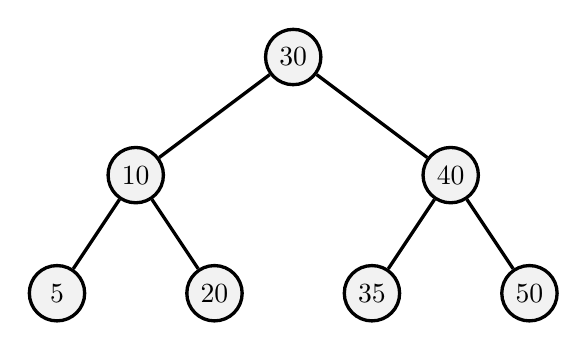
\begin{tikzpicture}[very thick,level/.style={sibling distance=40mm/#1}]
\tikzstyle{vertex}=[draw,fill=black!5,circle,minimum size=20pt,inner sep=1pt]
\node [vertex] (r){$30$}
  child {
	    node [vertex] (a) {$10$}
	    child {
		      node [vertex] {$5$}
	    }
	    child {
		      node [vertex] {$20$}
	    }
  }
  child {
	    node [vertex] {$40$}
	    child {
		      node [vertex] {$35$}
	    }
	    child {
		      node [vertex] {$50$}
	    }
  };
\end{tikzpicture}
&
\end{rcases} 
height = \log{(n)}
$$
\end{center}


\noindent
keys : 50, 40, 35, 30, 20, 10, 5


\begin{center}
$$
\begin{rcases}
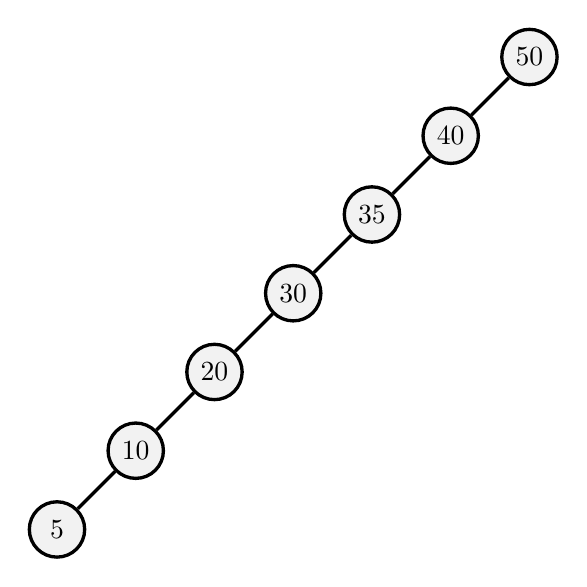
\begin{tikzpicture}[very thick,level/.style={sibling distance=20mm,level distance = 10mm}]
\tikzstyle{vertex}=[draw,fill=black!5,circle,minimum size=20pt,inner sep=1pt]
\node [vertex] (r){$50$}
  child {
	    node [vertex] (a) {$40$}
	    child {
		      node [vertex] {$35$}
		       child {
			      node [vertex] {$30$}
			      child {
				      node [vertex] {$20$}
				      child {
					      node [vertex] {$10$}
					      child {
						      node [vertex] {$5$}
					    } child [missing] {}
				    } child [missing] {}
			    } child [missing] {}
		    } child [missing] {}
	    } child [missing] {}
  } child [missing] {};
\end{tikzpicture}
&
\end{rcases} 
height = n
$$
\end{center}




\begin{tcolorbox}
Height of Binary Search Tree Depends on how keys are inserted
\end{tcolorbox}


\section{Can We Improve Binary Search Tree?}

Suppose we have 3 keys like : 30, 20, 10
\noindent
Then We Have These 5 following Shapes for making Binary Search Tree

\subsection{Order-1}
order : 30, 20, 10

\begin{center}
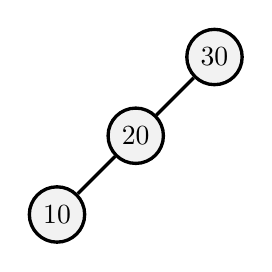
\begin{tikzpicture}[very thick,level/.style={sibling distance=20mm,level distance = 10mm}]
\tikzstyle{vertex}=[draw,fill=black!5,circle,minimum size=20pt,inner sep=1pt]
\node [vertex] (r){$30$}
  child {
	    node [vertex] (a) {$20$}
	    child {
		    	node [vertex] {$10$}
	    } child [missing] {}
  } child [missing] {};
\end{tikzpicture}
\end{center}

\subsection{Order-2}
order : 30, 10, 20

\begin{center}
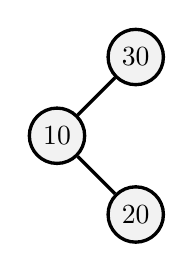
\begin{tikzpicture}[very thick,level/.style={sibling distance=20mm,level distance = 10mm}]
\tikzstyle{vertex}=[draw,fill=black!5,circle,minimum size=20pt,inner sep=1pt]
\node [vertex] (r){$30$}
  child {
	    node [vertex] (a) {$10$}
	    child [missing] {}
	    child {
		    	node [vertex] {$20$}
	    } 
  } child [missing] {};
\end{tikzpicture}
\end{center}

\subsection{Order-3}
order : 10, 30, 20

\begin{center}
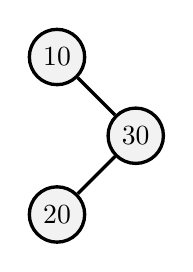
\begin{tikzpicture}[very thick,level/.style={sibling distance=20mm,level distance = 10mm}]
\tikzstyle{vertex}=[draw,fill=black!5,circle,minimum size=20pt,inner sep=1pt]
\node [vertex] (r){$10$}
  child [missing] {}
  child {
	    node [vertex] (a) {$30$}
	    child {
		    	node [vertex] {$20$}
	    } child [missing] {}
  };
\end{tikzpicture}
\end{center}

\subsection{Order-4}
order : 10, 20, 30

\begin{center}
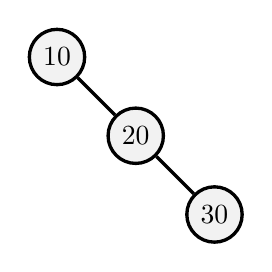
\begin{tikzpicture}[very thick,level/.style={sibling distance=20mm,level distance = 10mm}]
\tikzstyle{vertex}=[draw,fill=black!5,circle,minimum size=20pt,inner sep=1pt]
\node [vertex] (r){$10$}
  child [missing] {}
  child {
	    node [vertex] (a) {$20$}
	    child [missing] {}
	    child {
		    	node [vertex] {$30$}
	    } 
  };
\end{tikzpicture}
\end{center}

\subsection{Order-5}
order : 20, 10, 30 \qquad order : 20, 30, 10


\begin{center}
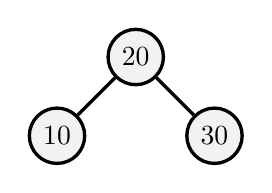
\begin{tikzpicture}[very thick,level/.style={sibling distance=20mm,level distance = 10mm}]
\tikzstyle{vertex}=[draw,fill=black!5,circle,minimum size=20pt,inner sep=1pt]
\node [vertex] (r){$20$}
  child {
  	    node [vertex] (a) {$10$}
  }
  child {
	    node [vertex] (a) {$30$}
  };
\end{tikzpicture}
\end{center}


\subsection{summary}

\begin{center}
  \bgroup
	  \def\arraystretch{1.5}%
	  \begin{tabular}{ c  c  c  }
	\qquad 30, 20, 10 \qquad\qquad &
	\qquad 30, 10, 20 \qquad\qquad &
	\qquad 10, 30, 20  \qquad\qquad \\
	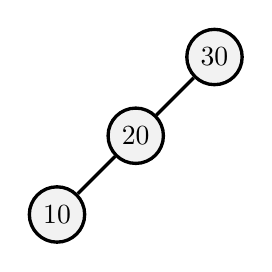
\begin{tikzpicture}[very thick,level/.style={sibling distance=20mm,level distance = 10mm}]
	\tikzstyle{vertex}=[draw,fill=black!5,circle,minimum size=20pt,inner sep=1pt]
	\node [vertex] (r){$30$}
	  child {
		    node [vertex] (a) {$20$}
		    child {
			    	node [vertex] {$10$}
		    } child [missing] {}
	  } child [missing] {};
	\end{tikzpicture}
 &

	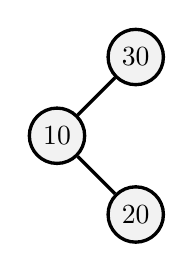
\begin{tikzpicture}[very thick,level/.style={sibling distance=20mm,level distance = 10mm}]
	\tikzstyle{vertex}=[draw,fill=black!5,circle,minimum size=20pt,inner sep=1pt]
	\node [vertex] (r){$30$}
	  child {
		    node [vertex] (a) {$10$}
		    child [missing] {}
		    child {
			    	node [vertex] {$20$}
		    } 
	  } child [missing] {};
	\end{tikzpicture}
 & 
	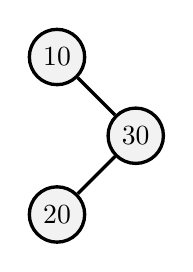
\begin{tikzpicture}[very thick,level/.style={sibling distance=20mm,level distance = 10mm}]
	\tikzstyle{vertex}=[draw,fill=black!5,circle,minimum size=20pt,inner sep=1pt]
	\node [vertex] (r){$10$}
	  child [missing] {}
	  child {
		    node [vertex] (a) {$30$}
		    child {
			    	node [vertex] {$20$}
		    } child [missing] {}
	  };
	\end{tikzpicture}
 \\ %\hline
 \\
    \qquad 10, 20, 30 \qquad &
    \multicolumn{2}{c}{20, 10, 30 \qquad 20, 30, 10}  \\
	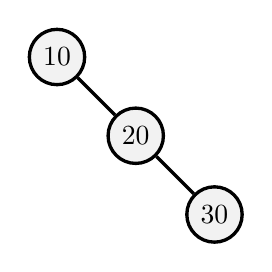
\begin{tikzpicture}[very thick,level/.style={sibling distance=20mm,level distance = 10mm}]
	\tikzstyle{vertex}=[draw,fill=black!5,circle,minimum size=20pt,inner sep=1pt]
	\node [vertex] (r){$10$}
	  child [missing] {}
	  child {
		    node [vertex] (a) {$20$}
		    child [missing] {}
		    child {
			    	node [vertex] {$30$}
		    } 
	  };
	\end{tikzpicture}
     & 
     \multicolumn{2}{c}{
	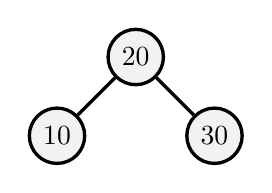
\begin{tikzpicture}[very thick,level/.style={sibling distance=20mm,level distance = 10mm}]
	\tikzstyle{vertex}=[draw,fill=black!5,circle,minimum size=20pt,inner sep=1pt]
	\node [vertex] (r){$20$}
	  child {
	  	    node [vertex] (a) {$10$}
	  }
	  child {
		    node [vertex] (a) {$30$}
	  };
	\end{tikzpicture} 
	}
 \\ %\hline
  \end{tabular}
  \egroup
\end{center}




\begin{tcolorbox}
Can We Improve Binay Search Tree?
\end{tcolorbox}

\begin{tcolorbox}
Is There Any Way to Convert The Order-[1-4] to Order-5 ?
\newline 
\noindent
Answer : Yes , We define Rotations
\end{tcolorbox}


\subsection{LL-Rotation}

\begin{center}
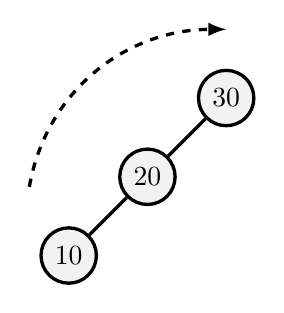
\begin{tikzpicture}[very thick,level/.style={sibling distance=20mm,level distance = 10mm}]
\tikzstyle{vertex}=[draw,fill=black!5,circle,minimum size=20pt,inner sep=1pt]
\node [vertex] (r) {$30$}
  child {
	    node [vertex] (a) {$20$}
	    child {
		    	node [vertex] (b) {$10$}
	    } child [missing] {}
  } child [missing] {};
  
\coordinate (A) at ([yshift=.5cm,xshift=-0.5cm]b.north);
%\coordinate (C) at ([yshift=.5cm,xshift=1cm]r);
\coordinate (C) at ([yshift=.5cm]r.north);

%\draw[dashed] plot[smooth] coordinates {(C) (A)};
\draw[->,>=latex,dashed] (A) to[out=80,in=180] (C);
\end{tikzpicture}
\end{center}


\subsection{RR-Rotation}



\begin{center}
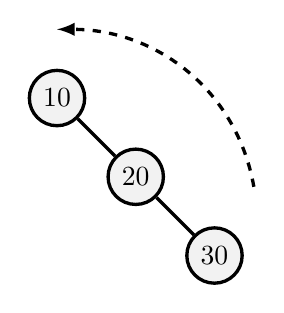
\begin{tikzpicture}[very thick,level/.style={sibling distance=20mm,level distance = 10mm}]
\tikzstyle{vertex}=[draw,fill=black!5,circle,minimum size=20pt,inner sep=1pt]
\node [vertex] (r){$10$}
  child [missing] {}
  child {
	    node [vertex] (a) {$20$}
	    child [missing] {}
	    child {
		    	node [vertex] (b) {$30$}
	    } 
  };
  

\coordinate (A) at ([yshift=.5cm,xshift=0.5cm]b.north);
\coordinate (C) at ([yshift=.5cm]r.north);
%\coordinate (C) at ([yshift=.5cm,xshift=-1cm]r);

%\draw[dashed] plot[smooth] coordinates {(C) (A)};
\draw[->,>=latex,dashed] (A) to[out=100,in=0] (C);
\end{tikzpicture}
\end{center}


\subsection{RL-Rotation}


\begin{center}
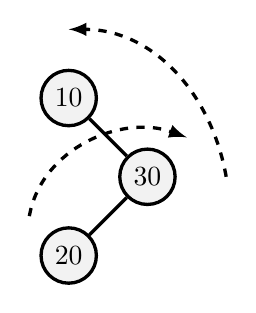
\begin{tikzpicture}[very thick,level/.style={sibling distance=20mm,level distance = 10mm}]
\tikzstyle{vertex}=[draw,fill=black!5,circle,minimum size=20pt,inner sep=1pt]
\node [vertex] (r){$10$}
  child [missing] {}
  child {
	    node [vertex] (a) {$30$}
	    child {
		    	node [vertex] (b) {$20$}
	    } child [missing] {}
  };
  
\coordinate (A) at ([xshift=1cm]a);
\coordinate (C) at ([yshift=.5cm]r.north);

\coordinate (E) at ([yshift=0.5cm,xshift=-0.5cm]b);
%\coordinate (F) at ([yshift=.5cm]a);
\coordinate (G) at ([xshift=0.5cm,yshift=0.5cm]a);

%\draw[dashed] plot[smooth] coordinates {(C) (A)};
\draw[->,>=latex,dashed] (A) to[out=100,in=0] (C);
\draw[->,>=latex,dashed] (E) to[out=80,in=160] (G) ;
\end{tikzpicture}
\end{center}


\subsection{LR-Rotation}


\begin{center}
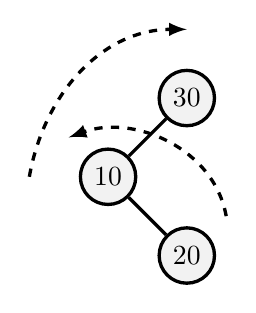
\begin{tikzpicture}[very thick,level/.style={sibling distance=20mm,level distance = 10mm}]
\tikzstyle{vertex}=[draw,fill=black!5,circle,minimum size=20pt,inner sep=1pt]
\node [vertex] (r){$30$}
  child {
	    node [vertex] (a) {$10$}
	    child [missing] {}
	    child {
		    	node [vertex] (b) {$20$}
	    } 
  } child [missing] {};
  
\coordinate (A) at ([xshift=-1cm]a);
\coordinate (C) at ([yshift=.5cm]r.north);

\coordinate (E) at ([yshift=0.5cm,xshift=0.5cm]b);
%\coordinate (F) at ([yshift=.5cm]a);
\coordinate (G) at ([xshift=-0.5cm,yshift=0.5cm]a);

%\draw[dashed] plot[smooth] coordinates {(C) (A)};
\draw[->,>=latex,dashed] (A) to[out=80,in=180] (C);
\draw[->,>=latex,dashed] (E) to[out=100,in=20] (G) ;
\end{tikzpicture}
\end{center}




\begin{tcolorbox}
There was only 3 Nodes What if we have Many Nodes ?
\end{tcolorbox}



\section{What is AVL Tree?}

AVL Tree is Height Balanced Binary Search Tree

\noindent
for balancing the height of Binary Search Tree we define One factor that is balance factor

\begin{tcolorbox}
\begin{center}
balance factor = height of left subtree - height of right subtree
\begin{gather*}
b_{f} = h_{l} - h_{r} = \{ -1 , 0 , 1 \} 
\\
\\
| b_{f} | = | h_{l} - h_{r} | \leq 1
\end{gather*}
\end{center}
\end{tcolorbox}



\subsection{Examples of finding balance factor of a node}



\begin{center}
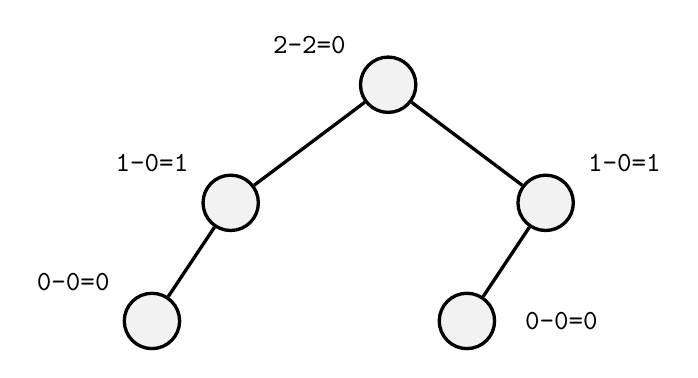
\begin{tikzpicture}[very thick,level/.style={sibling distance=40mm/#1}]
\tikzstyle{vertex}=[draw,fill=black!5,circle,minimum size=20pt,inner sep=1pt]
\tikzstyle{error}=[fill=red!60]
\node [vertex] (r){$$}
  child {
	    node [vertex] (a) {$$}
	    child {
		      node [vertex] (c) {$$}
	    } child [missing] {}
  }
  child {
	    node [vertex] (b) {$$}
	    child {
		      node [vertex] (d) {$$}
	    } child [missing] {}
};
% \normalsize\ttfamily
\node at (r) [xshift=-1cm,yshift=0.5cm] {\normalsize\ttfamily 2-2=0};
\node at (a) [xshift=-1cm,yshift=0.5cm] {\normalsize\ttfamily 1-0=1};
\node at (b) [xshift=1cm,yshift=0.5cm] {\normalsize\ttfamily 1-0=1};
\node at (c) [xshift=-1cm,yshift=0.5cm] {\normalsize\ttfamily 0-0=0};
\node at (d) [xshift=1.2cm,yshift=0cm] {\normalsize\ttfamily 0-0=0};

\end{tikzpicture}
\end{center}





\begin{center}
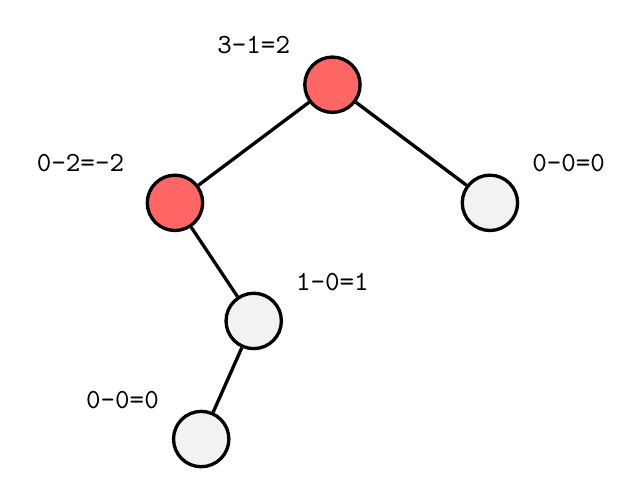
\begin{tikzpicture}[very thick,level/.style={sibling distance=40mm/#1}]
\tikzstyle{vertex}=[draw,fill=black!5,circle,minimum size=20pt,inner sep=1pt]
\tikzstyle{error}=[fill=red!60]
\node [vertex,error] (r){$$}
  child {
	    node [vertex,error] (a) {$$}
	    child [missing] {}
	    child {
		      node [vertex] (c) {$$}
		      child {
			      node [vertex] (e) {$$}
		   	 } child [missing] {}
	    } 
  }
  child {
	    node [vertex] (b) {$$}
};

\node at (r) [xshift=-1cm,yshift=0.5cm] {\normalsize\ttfamily 3-1=2};
\node at (a) [xshift=-1.2cm,yshift=0.5cm] {\normalsize\ttfamily 0-2=-2};
\node at (b) [xshift=1cm,yshift=0.5cm] {\normalsize\ttfamily 0-0=0};
\node at (c) [xshift=1cm,yshift=0.5cm] {\normalsize\ttfamily 1-0=1};
\node at (e) [xshift=-1cm,yshift=0.5cm] {\normalsize\ttfamily 0-0=0};

\end{tikzpicture}
\end{center}









\begin{center}
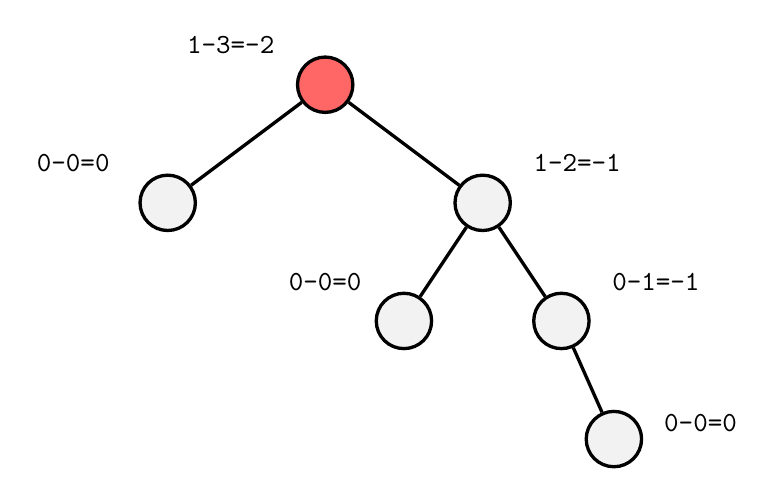
\begin{tikzpicture}[very thick,level/.style={sibling distance=40mm/#1}]
\tikzstyle{vertex}=[draw,fill=black!5,circle,minimum size=20pt,inner sep=1pt]
\tikzstyle{error}=[fill=red!60]
\node [vertex,error] (r){$$}
  child {
	    node [vertex] (a) {$$}
  }
  child {
	    node [vertex] (b) {$$}
	    child {
		      node [vertex] (c) {$$}
	    } 
	    child {
		      node [vertex] (d) {$$}
		      child [missing] {}
		      child {
			      node [vertex] (e) {$$}
		   	 } 
	    } 
};

\node at (r) [xshift=-1.2cm,yshift=0.5cm] {\normalsize\ttfamily 1-3=-2};
\node at (a) [xshift=-1.2cm,yshift=0.5cm] {\normalsize\ttfamily 0-0=0};
\node at (b) [xshift=1.2cm,yshift=0.5cm] {\normalsize\ttfamily 1-2=-1};
\node at (c) [xshift=-1cm,yshift=0.5cm] {\normalsize\ttfamily 0-0=0};
\node at (d) [xshift=1.2cm,yshift=0.5cm] {\normalsize\ttfamily 0-1=-1};
\node at (e) [xshift=1.1cm,yshift=0.2cm] {\normalsize\ttfamily 0-0=0};

\end{tikzpicture}
\end{center}




\section{Types Of Rotations}



\subsection{LL-Rotation}


\begin{center}
  \bgroup
  \def\arraystretch{1.5}%
  \begin{tabular}{ C  D  C }
   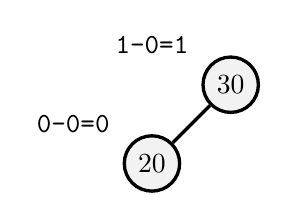
\begin{tikzpicture}[very thick,level/.style={sibling distance=20mm,level distance=10mm}]
\tikzstyle{vertex}=[draw,fill=black!5,circle,minimum size=20pt,inner sep=1pt]
\tikzstyle{error}=[fill=red!60]
\node [vertex] (r){$30$}
  child {
	    node [vertex] (a) {$20$}
  } child [missing] {}
  ;
\node at (r) [xshift=-1cm,yshift=0.5cm] {\normalsize\ttfamily 1-0=1};
\node at (a) [xshift=-1cm,yshift=0.5cm] {\normalsize\ttfamily 0-0=0}; 
\end{tikzpicture} & 
    
\begin{tikzpicture}[scale=2]
    \draw (0,0) node (arrow) 
{$\xRightarrow{\text{\normalsize\ttfamily insert 10}}$};
    \end{tikzpicture} &
    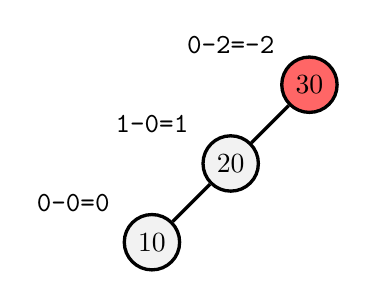
\begin{tikzpicture}[very thick,level/.style={sibling distance=20mm,level distance=10mm}]
\tikzstyle{vertex}=[draw,fill=black!5,circle,minimum size=20pt,inner sep=1pt]
\tikzstyle{error}=[fill=red!60]
    \node [vertex,error] (r){$30$}
  child {
	    node [vertex] (a) {$20$}
	     child {
		    node [vertex] (b) {$10$}
	     } child [missing] {}
  } child [missing] {}
  ;

\node at (r) [xshift=-1cm,yshift=0.5cm] {\normalsize\ttfamily 0-2=-2};
\node at (a) [xshift=-1cm,yshift=0.5cm] {\normalsize\ttfamily 1-0=1};
\node at (b) [xshift=-1cm,yshift=0.5cm] {\normalsize\ttfamily 0-0=0};
\end{tikzpicture}
  \end{tabular}
  \egroup
\end{center}

\begin{tcolorbox}
\tikz \node[vertex,error] {$30$} ;
became unbalanced because we insert 
\tikz \node[vertex] {$10$} ;
at left and left so we called it LL-Rotation .
\end{tcolorbox}






\begin{center}
  \bgroup
  \def\arraystretch{1.5}%
  \begin{tabular}{ C  D  C }
  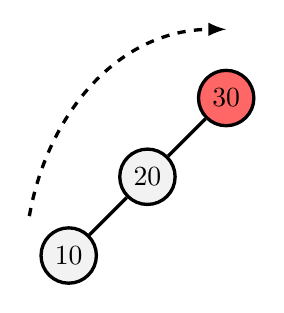
\begin{tikzpicture}[very thick,level/.style={sibling distance=20mm,level distance=10mm}]
\tikzstyle{vertex}=[draw,fill=black!5,circle,minimum size=20pt,inner sep=1pt]
\tikzstyle{error}=[fill=red!60]
    \node [vertex,error] (r){$30$}
  child {
	    node [vertex] (a) {$20$}
	     child {
		    node [vertex] (b) {$10$}
	     } child [missing] {}
  } child [missing] {}
  ;
\coordinate (A) at ([yshift=.5cm,xshift=-0.5cm]b);
\coordinate (C) at ([yshift=.5cm]r.north);
%\coordinate (C) at ([yshift=.5cm,xshift=-1cm]r);

%\draw[dashed] plot[smooth] coordinates {(C) (A)};
\draw[->,>=latex,dashed] (A) to[out=80,in=180] (C);
\end{tikzpicture}
   & 
    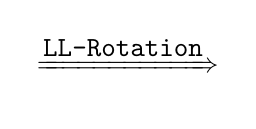
\begin{tikzpicture}[scale=2]
    \draw (0,0) node (arrow) 
{$\xRightarrow{\text{\normalsize\ttfamily LL-Rotation}}$};
    \end{tikzpicture} &
    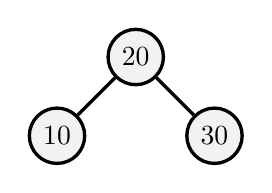
\begin{tikzpicture}[very thick,level/.style={sibling distance=20mm,level distance=10mm}]
\tikzstyle{vertex}=[draw,fill=black!5,circle,minimum size=20pt,inner sep=1pt]
\tikzstyle{error}=[fill=red!60]
    \node [vertex] (r){$20$}
  child {
	    node [vertex] (a) {$10$}
  } child {
  		node [vertex] (b) {$30$}
  }
  ;
\end{tikzpicture}
  \end{tabular}
  \egroup
\end{center}


\subsection{RR-Rotation}




\begin{center}
  \bgroup
  \def\arraystretch{1.5}%
  \begin{tabular}{ C  D  C }
   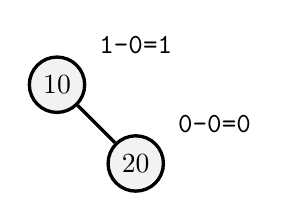
\begin{tikzpicture}[very thick,level/.style={sibling distance=20mm,level distance=10mm}]
\tikzstyle{vertex}=[draw,fill=black!5,circle,minimum size=20pt,inner sep=1pt]
\tikzstyle{error}=[fill=red!60]
\node [vertex] (r){$10$}
  child [missing] {}
  child {
	    node [vertex] (a) {$20$}
  } 
  ;

\node at (r) [xshift=1cm,yshift=0.5cm] {\normalsize\ttfamily 1-0=1};
\node at (a) [xshift=1cm,yshift=0.5cm] {\normalsize\ttfamily 0-0=0}; 
\end{tikzpicture} & 
    
\begin{tikzpicture}[scale=2]
    \draw (0,0) node (arrow) 
{$\xRightarrow{\text{\normalsize\ttfamily insert 30}}$};
    \end{tikzpicture} &
    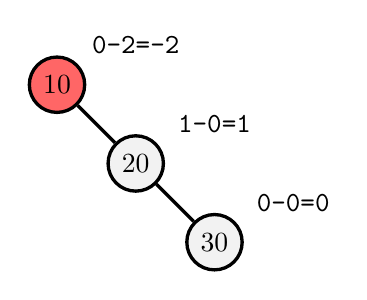
\begin{tikzpicture}[very thick,level/.style={sibling distance=20mm,level distance=10mm}]
\tikzstyle{vertex}=[draw,fill=black!5,circle,minimum size=20pt,inner sep=1pt]
\tikzstyle{error}=[fill=red!60]
    \node [vertex,error] (r){$10$}
    child [missing] {}
  child {
	    node [vertex] (a) {$20$}
	    child [missing] {}
	     child {
		    node [vertex] (b) {$30$}
	     } 
  } 
  ;

\node at (r) [xshift=1cm,yshift=0.5cm] {\normalsize\ttfamily 0-2=-2};
\node at (a) [xshift=1cm,yshift=0.5cm] {\normalsize\ttfamily 1-0=1};
\node at (b) [xshift=1cm,yshift=0.5cm] {\normalsize\ttfamily 0-0=0};
\end{tikzpicture}
  \end{tabular}
  \egroup
\end{center}

\begin{tcolorbox}
\tikz \node[vertex,error] {$10$} ;
became unbalanced because we insert 
\tikz \node[vertex] {$30$} ;
at right and right so we called it RR-Rotation .
\end{tcolorbox}






\begin{center}
  \bgroup
  \def\arraystretch{1.5}%
  \begin{tabular}{ C  D  C }
  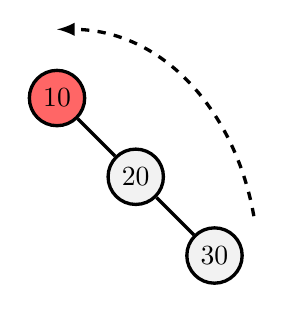
\begin{tikzpicture}[very thick,level/.style={sibling distance=20mm,level distance=10mm}]
\tikzstyle{vertex}=[draw,fill=black!5,circle,minimum size=20pt,inner sep=1pt]
\tikzstyle{error}=[fill=red!60]
    \node [vertex,error] (r){$10$}
    child [missing] {}
  child {
	    node [vertex] (a) {$20$}
	    child [missing] {}
	     child {
		    node [vertex] (b) {$30$}
	     } 
  } 
  ;
\coordinate (A) at ([yshift=.5cm,xshift=0.5cm]b);
%\coordinate (C) at ([yshift=.5cm,xshift=1cm]r);
\coordinate (C) at ([yshift=.5cm]r.north);

%\draw[dashed] plot[smooth] coordinates {(C) (A)};
\draw[->,>=latex,dashed] (A) to[out=100,in=0] (C);
\end{tikzpicture}
   & 
    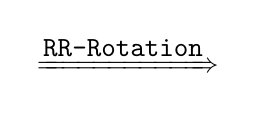
\begin{tikzpicture}[scale=2]
    \draw (0,0) node (arrow) 
{$\xRightarrow{\text{\normalsize\ttfamily RR-Rotation}}$};
    \end{tikzpicture} &
    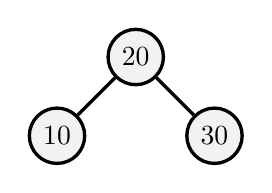
\begin{tikzpicture}[very thick,level/.style={sibling distance=20mm,level distance=10mm}]
\tikzstyle{vertex}=[draw,fill=black!5,circle,minimum size=20pt,inner sep=1pt]
\tikzstyle{error}=[fill=red!60]
    \node [vertex] (r){$20$}
  child {
	    node [vertex] (a) {$10$}
  } child {
  		node [vertex] (b) {$30$}
  }
  ;
\end{tikzpicture}
  \end{tabular}
  \egroup
\end{center}




\subsection{LR-Rotation}


\begin{center}
  \bgroup
  \def\arraystretch{1.5}%
  \begin{tabular}{ C  D  C }
   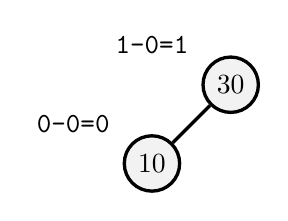
\begin{tikzpicture}[very thick,level/.style={sibling distance=20mm,level distance=10mm}]
\tikzstyle{vertex}=[draw,fill=black!5,circle,minimum size=20pt,inner sep=1pt]
\tikzstyle{error}=[fill=red!60]
\node [vertex] (r){$30$}
  child {
	    node [vertex] (a) {$10$}
  } child [missing] {}
  ;

\node at (r) [xshift=-1cm,yshift=0.5cm] {\normalsize\ttfamily 1-0=1};
\node at (a) [xshift=-1cm,yshift=0.5cm] {\normalsize\ttfamily 0-0=0}; 
\end{tikzpicture} & 
    
\begin{tikzpicture}[scale=2]
    \draw (0,0) node (arrow) 
{$\xRightarrow{\text{\normalsize\ttfamily insert 20}}$};
    \end{tikzpicture} &
    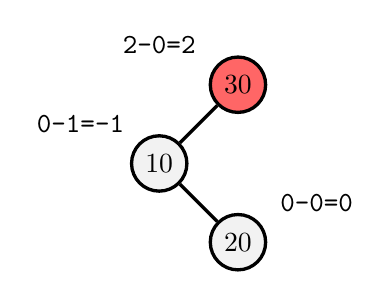
\begin{tikzpicture}[very thick,level/.style={sibling distance=20mm,level distance=10mm}]
\tikzstyle{vertex}=[draw,fill=black!5,circle,minimum size=20pt,inner sep=1pt]
\tikzstyle{error}=[fill=red!60]
    \node [vertex,error] (r){$30$}
  child {
	    node [vertex] (a) {$10$}
	    child [missing] {}
	     child {
		    node [vertex] (b) {$20$}
	     } 
  } child [missing] {}
  ;

\node at (r) [xshift=-1cm,yshift=0.5cm] {\normalsize\ttfamily 2-0=2};
\node at (a) [xshift=-1cm,yshift=0.5cm] {\normalsize\ttfamily 0-1=-1};
\node at (b) [xshift=1cm,yshift=0.5cm] {\normalsize\ttfamily 0-0=0};
\end{tikzpicture}
  \end{tabular}
  \egroup
\end{center}



\begin{tcolorbox}
\tikz \node[vertex,error] {$30$} ;
became imbalanced because we insert 
\tikz \node[vertex] {$20$} ;
at left then right so we called it LR-Rotation .
\end{tcolorbox}





\begin{center}
  \bgroup
  \def\arraystretch{1.5}%
  \begin{tabular}{ C  D  C }
   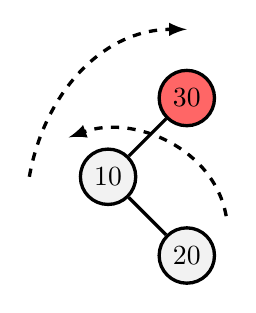
\begin{tikzpicture}[very thick,level/.style={sibling distance=20mm,level distance=10mm}]
\tikzstyle{vertex}=[draw,fill=black!5,circle,minimum size=20pt,inner sep=1pt]
\tikzstyle{error}=[fill=red!60]
    \node [vertex,error] (r){$30$}
  child {
	    node [vertex] (a) {$10$}
	    child [missing] {}
	     child {
		    node [vertex] (b) {$20$}
	     } 
  } child [missing] {}
  ;
  \coordinate (A) at ([xshift=-1cm]a);
\coordinate (C) at ([yshift=.5cm]r.north);

\coordinate (E) at ([yshift=0.5cm,xshift=0.5cm]b);
%\coordinate (F) at ([yshift=.5cm]a);
\coordinate (G) at ([xshift=-0.5cm,yshift=0.5cm]a);

%\draw[dashed] plot[smooth] coordinates {(C) (A)};
\draw[->,>=latex,dashed] (A) to[out=80,in=180] (C);
\draw[->,>=latex,dashed] (E) to[out=100,in=20] (G) ;
\end{tikzpicture} & 
    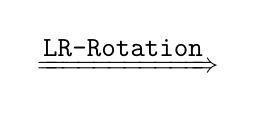
\begin{tikzpicture}[scale=2]
    \draw (0,0) node (arrow) 
{$\xRightarrow{\text{\normalsize\ttfamily LR-Rotation}}$};
    \end{tikzpicture} &
    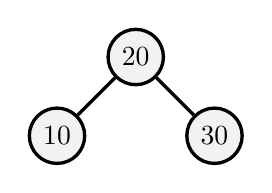
\begin{tikzpicture}[very thick,level/.style={sibling distance=20mm,level distance=10mm}]
\tikzstyle{vertex}=[draw,fill=black!5,circle,minimum size=20pt,inner sep=1pt]
\tikzstyle{error}=[fill=red!60]
    \node [vertex] (r){$20$}
  child {
	    node [vertex] (a) {$10$}
  } child {
  		node [vertex] (b) {$30$}
  }
  ;
\end{tikzpicture}
  \end{tabular}
  \egroup
\end{center}



\subsection{RL-Rotation}



\begin{center}
  \bgroup
  \def\arraystretch{1.5}%
  \begin{tabular}{ C  D  C }
   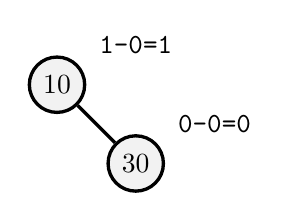
\begin{tikzpicture}[very thick,level/.style={sibling distance=20mm,level distance=10mm}]
\tikzstyle{vertex}=[draw,fill=black!5,circle,minimum size=20pt,inner sep=1pt]
\tikzstyle{error}=[fill=red!60]
\node [vertex] (r){$10$}
  child [missing] {}
  child {
	    node [vertex] (a) {$30$}
  };
\node at (r) [xshift=1cm,yshift=0.5cm] {\normalsize\ttfamily 1-0=1};
\node at (a) [xshift=1cm,yshift=0.5cm] {\normalsize\ttfamily 0-0=0};
\end{tikzpicture} & 
    
\begin{tikzpicture}[scale=2]
    \draw (0,0) node (arrow) 
{$\xRightarrow{\text{\normalsize\ttfamily insert 20}}$};
    \end{tikzpicture} &
    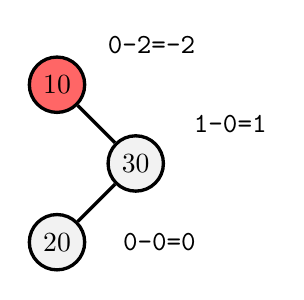
\begin{tikzpicture}[very thick,level/.style={sibling distance=20mm,level distance=10mm}]
\tikzstyle{vertex}=[draw,fill=black!5,circle,minimum size=20pt,inner sep=1pt]
\tikzstyle{error}=[fill=red!60]
    \node [vertex,error] (r){$10$}
    child [missing] {}
  child {
	    node [vertex] (a) {$30$}
	     child {
		    node [vertex] (b) {$20$}
	     }  child [missing] {}
  } 
  ;

\node at (r) [xshift=1.2cm,yshift=0.5cm] {\normalsize\ttfamily 0-2=-2};
\node at (a) [xshift=1.2cm,yshift=0.5cm] {\normalsize\ttfamily 1-0=1};
\node at (b) [xshift=1.3cm,yshift=0cm] {\normalsize\ttfamily 0-0=0};
\end{tikzpicture}
  \end{tabular}
  \egroup
\end{center}



\begin{tcolorbox}
\tikz \node[vertex,error] {$10$} ;
became unbalanced because we insert 
\tikz \node[vertex] {$20$} ;
at right and right so we called it RR-Rotation .
\end{tcolorbox}






\begin{center}
  \bgroup
  \def\arraystretch{1.5}%
  \begin{tabular}{ C  D  C }
  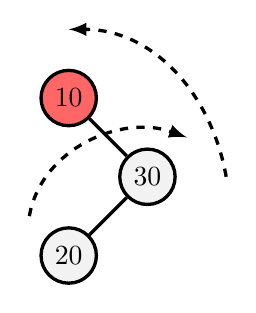
\begin{tikzpicture}[very thick,level/.style={sibling distance=20mm,level distance=10mm}]
\tikzstyle{vertex}=[draw,fill=black!5,circle,minimum size=20pt,inner sep=1pt]
\tikzstyle{error}=[fill=red!60]
    \node [vertex,error] (r){$10$}
    child [missing] {}
  child {
	    node [vertex] (a) {$30$}
	     child {
		    node [vertex] (b) {$20$}
	     } child [missing] {}
  } 
  ;
\coordinate (A) at ([xshift=1cm]a);
\coordinate (C) at ([yshift=.5cm]r.north);

\coordinate (E) at ([yshift=0.5cm,xshift=-0.5cm]b);
%\coordinate (F) at ([yshift=.5cm]a);
\coordinate (G) at ([xshift=0.5cm,yshift=0.5cm]a);

%\draw[dashed] plot[smooth] coordinates {(C) (A)};
\draw[->,>=latex,dashed] (A) to[out=100,in=0] (C);
\draw[->,>=latex,dashed] (E) to[out=80,in=160] (G) ;
\end{tikzpicture}
   & 
    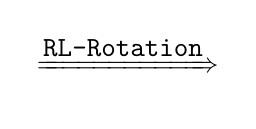
\begin{tikzpicture}[scale=2]
    \draw (0,0) node (arrow) 
{$\xRightarrow{\text{\normalsize\ttfamily RL-Rotation}}$};
    \end{tikzpicture} &
    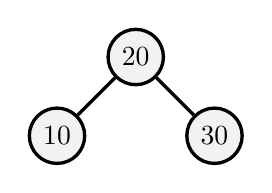
\begin{tikzpicture}[very thick,level/.style={sibling distance=20mm,level distance=10mm}]
\tikzstyle{vertex}=[draw,fill=black!5,circle,minimum size=20pt,inner sep=1pt]
\tikzstyle{error}=[fill=red!60]
    \node [vertex] (r){$20$}
  child {
	    node [vertex] (a) {$10$}
  } child {
  		node [vertex] (b) {$30$}
  }
  ;
\end{tikzpicture}
  \end{tabular}
  \egroup
\end{center}



\section{Rotations With Sub-Trees}


\subsection{LL-Rotation With Sub-Trees}

\begin{center}
  \bgroup
  \def\arraystretch{1.5}%
  \begin{tabular}{ E G E G }
   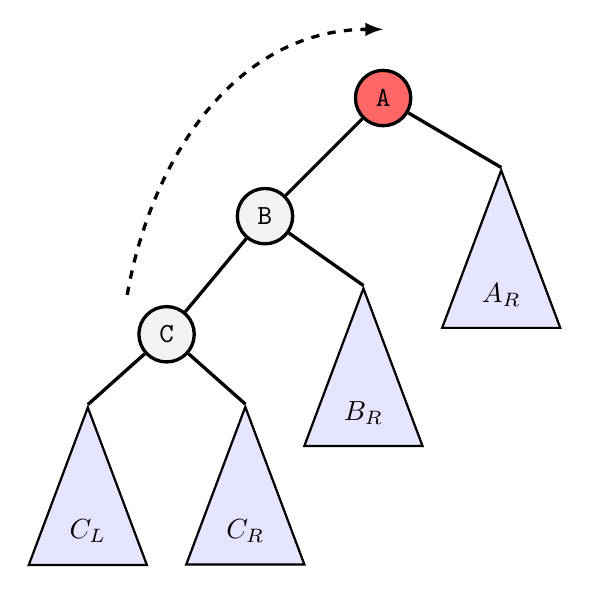
\begin{tikzpicture}[
 very thick,
  level/.style={sibling distance=40mm/#1,level distance=10mm}
  inner/.style={fill = light blue,circle,draw,thick,minimum width=5mm,inner sep=0},
  small inner/.style={inner,minimum width = 3mm},
  triangle/.style={fill = light blue,isosceles triangle,draw=,thick,shape border rotate=90,isosceles triangle stretches=true, minimum height=20mm,minimum width=15mm,inner sep=0,yshift={-10mm}},
  small triangle/.style={triangle, minimum height = 8mm, minimum width = 6mm },
  large triangle/.style={triangle,minimum width = 27mm,minimum height=36mm,yshift={-11mm}},
  very large triangle/.style={triangle,minimum width = 33mm,minimum height=44mm,yshift={-11mm}},
  level 1/.style={sibling distance=30mm},
  level 2/.style={sibling distance=25mm},
  level 3/.style={sibling distance=20mm},
  %level 4/.style={sibling distance=25mm},
  %level 4/.style={sibling distance=15mm},
  %level 5/.style={sibling distance=7mm},
]
\tikzstyle{vertex}=[draw,fill=black!5,circle,minimum size=20pt,inner sep=1pt]
\tikzstyle{error}=[fill=red!60]
  \colorlet{light blue}{blue!10}
  \node[vertex,error] (r) {\normalsize\ttfamily A}
    child {
       node [vertex] (a) {\normalsize\ttfamily B }
       child  {
       	node [vertex] (b) {\normalsize\ttfamily C }
       	child [child anchor=north]  {
       	    node [triangle] { $C_{L}$ }
	     } child [child anchor=north] {
	        node [triangle] { $C_{R}$ }
	     }
	  } child [child anchor=north] {
	      node [triangle] { $B_{R}$ }
	  }
    } child [child anchor=north] {
         node [triangle] { $A_{R}$ }
    }
    ;
    \coordinate (A) at ([yshift=.5cm,xshift=-0.5cm]b);
\coordinate (C) at ([yshift=.5cm]r.north);
%\coordinate (C) at ([yshift=.5cm,xshift=-1cm]r);

%\draw[dashed] plot[smooth] coordinates {(C) (A)};
\draw[->,>=latex,dashed] (A) to[out=80,in=180] (C);
\end{tikzpicture} & 
    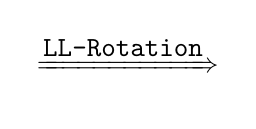
\begin{tikzpicture}
    \draw (0,0) node (arrow) 
{$\xRightarrow{\text{\normalsize\ttfamily LL-Rotation}}$};
    \end{tikzpicture}  &
    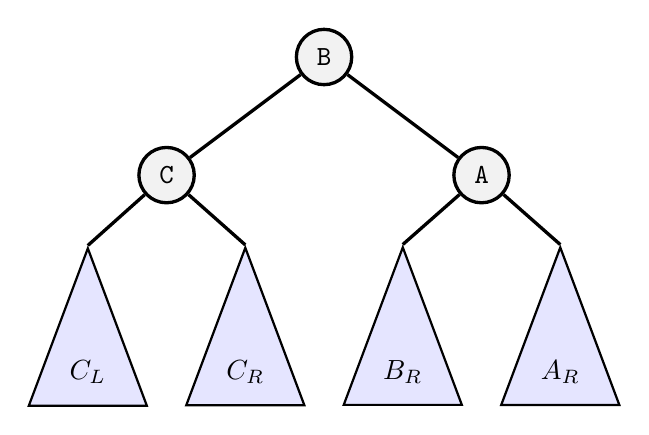
\begin{tikzpicture}[
 very thick,
  level/.style={sibling distance=40mm/#1,level distance=10mm}
  inner/.style={fill = light blue,circle,draw,thick,minimum width=5mm,inner sep=0},
  small inner/.style={inner,minimum width = 3mm},
  triangle/.style={fill = light blue,isosceles triangle,draw=,thick,shape border rotate=90,isosceles triangle stretches=true, minimum height=20mm,minimum width=15mm,inner sep=0,yshift={-10mm}},
  small triangle/.style={triangle, minimum height = 8mm, minimum width = 6mm },
  large triangle/.style={triangle,minimum width = 27mm,minimum height=36mm,yshift={-11mm}},
  very large triangle/.style={triangle,minimum width = 33mm,minimum height=44mm,yshift={-11mm}},
  level 1/.style={sibling distance=40mm},
  level 2/.style={sibling distance=20mm},
  level 3/.style={sibling distance=20mm},
  %level 4/.style={sibling distance=25mm},
  %level 4/.style={sibling distance=15mm},
  %level 5/.style={sibling distance=7mm},
]
\tikzstyle{vertex}=[draw,fill=black!5,circle,minimum size=20pt,inner sep=1pt]
\tikzstyle{error}=[fill=red!60]
  \colorlet{light blue}{blue!10}
  \node[vertex] (r) {\normalsize\ttfamily B}
    child {
       node [vertex] {\normalsize\ttfamily C }
       	child [child anchor=north]  {
       	    node [triangle] { $C_{L}$ }
	     } child [child anchor=north] {
	        node [triangle] { $C_{R}$ }
	     }
    } child {
         node [vertex] {\normalsize\ttfamily A }
         child [child anchor=north] {
         node [triangle] { $B_{R}$ }
         }
         child [child anchor=north] {
         node [triangle] { $A_{R}$ }
         }
    }
    ;
\end{tikzpicture} 
   &
     \\ 
  \end{tabular}
  \egroup
\end{center}




\subsection{RR-Rotation With Sub-Trees}




\begin{center}
  \bgroup
  \def\arraystretch{1.5}%
  \begin{tabular}{ E G E G }
   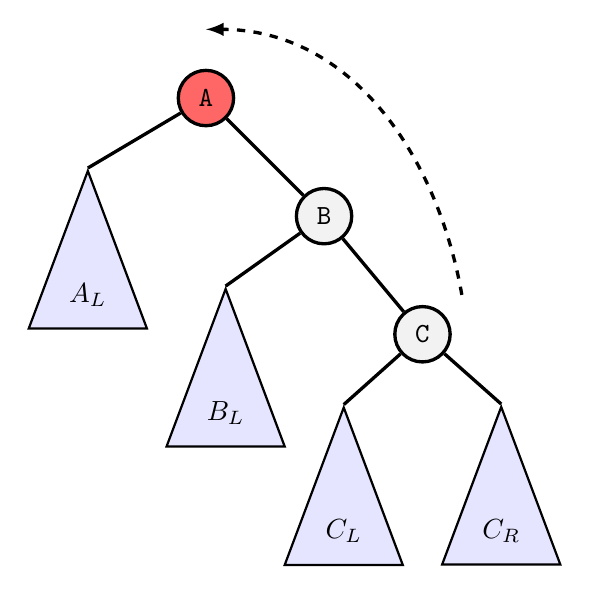
\begin{tikzpicture}[
 very thick,
  level/.style={sibling distance=40mm/#1,level distance=10mm}
  inner/.style={fill = light blue,circle,draw,thick,minimum width=5mm,inner sep=0},
  small inner/.style={inner,minimum width = 3mm},
  triangle/.style={fill = light blue,isosceles triangle,draw=,thick,shape border rotate=90,isosceles triangle stretches=true, minimum height=20mm,minimum width=15mm,inner sep=0,yshift={-10mm}},
  small triangle/.style={triangle, minimum height = 8mm, minimum width = 6mm },
  large triangle/.style={triangle,minimum width = 27mm,minimum height=36mm,yshift={-11mm}},
  very large triangle/.style={triangle,minimum width = 33mm,minimum height=44mm,yshift={-11mm}},
  level 1/.style={sibling distance=30mm},
  level 2/.style={sibling distance=25mm},
  level 3/.style={sibling distance=20mm},
  %level 4/.style={sibling distance=25mm},
  %level 4/.style={sibling distance=15mm},
  %level 5/.style={sibling distance=7mm},
]
\tikzstyle{vertex}=[draw,fill=black!5,circle,minimum size=20pt,inner sep=1pt]
\tikzstyle{error}=[fill=red!60]
  \colorlet{light blue}{blue!10}
  \node[vertex,error] (r) {\normalsize\ttfamily A}
  child [child anchor=north] {
         node [triangle] { $A_{L}$ }
    }
    child {
       node [vertex] (a) {\normalsize\ttfamily B }
       child [child anchor=north] {
	      node [triangle] { $B_{L}$ }
	  }
       child  {
       	node [vertex] (b) {\normalsize\ttfamily C }
       	child [child anchor=north]  {
       	    node [triangle] { $C_{L}$ }
	     } child [child anchor=north] {
	        node [triangle] { $C_{R}$ }
	     }
	  } 
    } 
    ;
\coordinate (A) at ([yshift=.5cm,xshift=0.5cm]b);
%\coordinate (C) at ([yshift=.5cm,xshift=1cm]r);
\coordinate (C) at ([yshift=.5cm]r.north);

%\draw[dashed] plot[smooth] coordinates {(C) (A)};
\draw[->,>=latex,dashed] (A) to[out=100,in=0] (C);
\end{tikzpicture} & 
    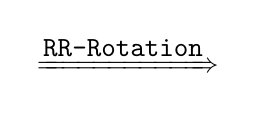
\begin{tikzpicture}
    \draw (0,0) node (arrow) 
{$\xRightarrow{\text{\normalsize\ttfamily RR-Rotation}}$};
    \end{tikzpicture}  &
    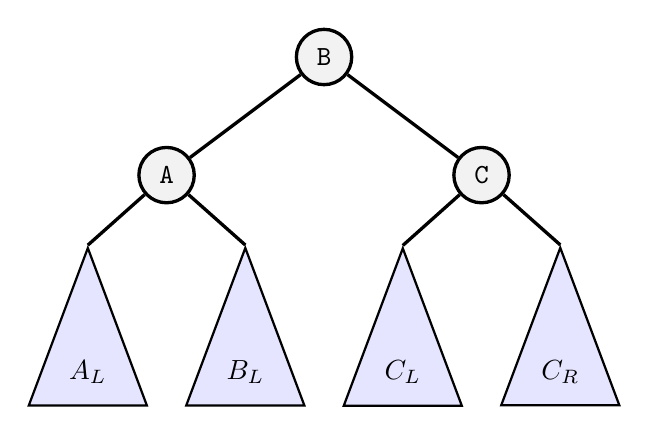
\begin{tikzpicture}[
 very thick,
  level/.style={sibling distance=40mm/#1,level distance=10mm}
  inner/.style={fill = light blue,circle,draw,thick,minimum width=5mm,inner sep=0},
  small inner/.style={inner,minimum width = 3mm},
  triangle/.style={fill = light blue,isosceles triangle,draw=,thick,shape border rotate=90,isosceles triangle stretches=true, minimum height=20mm,minimum width=15mm,inner sep=0,yshift={-10mm}},
  small triangle/.style={triangle, minimum height = 8mm, minimum width = 6mm },
  large triangle/.style={triangle,minimum width = 27mm,minimum height=36mm,yshift={-11mm}},
  very large triangle/.style={triangle,minimum width = 33mm,minimum height=44mm,yshift={-11mm}},
  level 1/.style={sibling distance=40mm},
  level 2/.style={sibling distance=20mm},
  level 3/.style={sibling distance=20mm},
  %level 4/.style={sibling distance=25mm},
  %level 4/.style={sibling distance=15mm},
  %level 5/.style={sibling distance=7mm},
]
\tikzstyle{vertex}=[draw,fill=black!5,circle,minimum size=20pt,inner sep=1pt]
\tikzstyle{error}=[fill=red!60]
  \colorlet{light blue}{blue!10}
  \node[vertex] (r) {\normalsize\ttfamily B}
    child {
       node [vertex] {\normalsize\ttfamily A }
       	child [child anchor=north]  {
       	    node [triangle] { $A_{L}$ }
	     } child [child anchor=north] {
	        node [triangle] { $B_{L}$ }
	     }
    } child {
         node [vertex] {\normalsize\ttfamily C }
         child [child anchor=north] {
         node [triangle] { $C_{L}$ }
         }
         child [child anchor=north] {
         node [triangle] { $C_{R}$ }
         }
    }
    ;
\end{tikzpicture} 
&
     \\ 
  \end{tabular}
  \egroup
\end{center}




\subsection{RL-Rotation With Sub-Trees}




\begin{center}
  \bgroup
  \def\arraystretch{1.5}%
  \begin{tabular}{ E G E G }
   \begin{tikzpicture}[
 very thick,
  level/.style={sibling distance=40mm/#1,level distance=10mm}
  inner/.style={fill = light blue,circle,draw,thick,minimum width=5mm,inner sep=0},
  small inner/.style={inner,minimum width = 3mm},
  triangle/.style={fill = light blue,isosceles triangle,draw=,thick,shape border rotate=90,isosceles triangle stretches=true, minimum height=20mm,minimum width=15mm,inner sep=0,yshift={-10mm}},
  small triangle/.style={triangle, minimum height = 8mm, minimum width = 6mm },
  large triangle/.style={triangle,minimum width = 27mm,minimum height=36mm,yshift={-11mm}},
  very large triangle/.style={triangle,minimum width = 33mm,minimum height=44mm,yshift={-11mm}},
  level 1/.style={sibling distance=30mm},
  level 2/.style={sibling distance=25mm},
  level 3/.style={sibling distance=20mm},
  %level 4/.style={sibling distance=25mm},
  %level 4/.style={sibling distance=15mm},
  %level 5/.style={sibling distance=7mm},
]
\tikzstyle{vertex}=[draw,fill=black!5,circle,minimum size=20pt,inner sep=1pt]
\tikzstyle{error}=[fill=red!60]
  \colorlet{light blue}{blue!10}
  \node[vertex,error] (r) {\normalsize\ttfamily A}
  child {
       node [vertex] (a) {\normalsize\ttfamily B }
       child [child anchor=north] {
	      node [triangle] { $B_{L}$ }
	  }
       child  {
       	node [vertex] (b) {\normalsize\ttfamily C }
       	child [child anchor=north]  {
       	    node [triangle] { $C_{L}$ }
	     } child [child anchor=north] {
	        node [triangle] { $C_{R}$ }
	     }
	  } 
    } 
  child [child anchor=north] {
         node [triangle] { $A_{R}$ }
    }
    
    ;
  \coordinate (A) at ([xshift=-1cm]a);
\coordinate (C) at ([yshift=.5cm]r.north);

\coordinate (E) at ([yshift=0.5cm,xshift=0.5cm]b);
%\coordinate (F) at ([yshift=.5cm]a);
\coordinate (G) at ([xshift=-0.5cm,yshift=0.5cm]a);

%\draw[dashed] plot[smooth] coordinates {(C) (A)};
\draw[->,>=latex,dashed] (A) to[out=80,in=180] (C);
\draw[->,>=latex,dashed] (E) to[out=100,in=20] (G) ;
\end{tikzpicture} & 
    \begin{tikzpicture}
    \draw (0,0) node (arrow) 
{$\xRightarrow{\text{\normalsize\ttfamily LR-Rotation}}$};
    \end{tikzpicture}  &
    \begin{tikzpicture}[
 very thick,
  level/.style={sibling distance=40mm/#1,level distance=10mm}
  inner/.style={fill = light blue,circle,draw,thick,minimum width=5mm,inner sep=0},
  small inner/.style={inner,minimum width = 3mm},
  triangle/.style={fill = light blue,isosceles triangle,draw=,thick,shape border rotate=90,isosceles triangle stretches=true, minimum height=20mm,minimum width=15mm,inner sep=0,yshift={-10mm}},
  small triangle/.style={triangle, minimum height = 8mm, minimum width = 6mm },
  large triangle/.style={triangle,minimum width = 27mm,minimum height=36mm,yshift={-11mm}},
  very large triangle/.style={triangle,minimum width = 33mm,minimum height=44mm,yshift={-11mm}},
  level 1/.style={sibling distance=40mm},
  level 2/.style={sibling distance=20mm},
  level 3/.style={sibling distance=20mm},
  %level 4/.style={sibling distance=25mm},
  %level 4/.style={sibling distance=15mm},
  %level 5/.style={sibling distance=7mm},
]
\tikzstyle{vertex}=[draw,fill=black!5,circle,minimum size=20pt,inner sep=1pt]
\tikzstyle{error}=[fill=red!60]
  \colorlet{light blue}{blue!10}
  \node[vertex] (r) {\normalsize\ttfamily C}
    child {
       node [vertex] {\normalsize\ttfamily B }
       	child [child anchor=north]  {
       	    node [triangle] { $B_{L}$ }
	     } child [child anchor=north] {
	        node [triangle] { $C_{L}$ }
	     }
    } child {
         node [vertex] {\normalsize\ttfamily A }
         child [child anchor=north] {
         node [triangle] { $C_{R}$ }
         }
         child [child anchor=north] {
         node [triangle] { $A_{R}$ }
         }
    }
    ;
\end{tikzpicture} 
&
     \\ 
  \end{tabular}
  \egroup
\end{center}


\subsection{LR-Rotation With Sub-Trees}




\begin{center}
  \bgroup
  \def\arraystretch{1.5}%
  \begin{tabular}{ E G E G }
   \begin{tikzpicture}[
 very thick,
  level/.style={sibling distance=40mm/#1,level distance=10mm}
  inner/.style={fill = light blue,circle,draw,thick,minimum width=5mm,inner sep=0},
  small inner/.style={inner,minimum width = 3mm},
  triangle/.style={fill = light blue,isosceles triangle,draw=,thick,shape border rotate=90,isosceles triangle stretches=true, minimum height=20mm,minimum width=15mm,inner sep=0,yshift={-10mm}},
  small triangle/.style={triangle, minimum height = 8mm, minimum width = 6mm },
  large triangle/.style={triangle,minimum width = 27mm,minimum height=36mm,yshift={-11mm}},
  very large triangle/.style={triangle,minimum width = 33mm,minimum height=44mm,yshift={-11mm}},
  level 1/.style={sibling distance=30mm},
  level 2/.style={sibling distance=25mm},
  level 3/.style={sibling distance=20mm},
  %level 4/.style={sibling distance=25mm},
  %level 4/.style={sibling distance=15mm},
  %level 5/.style={sibling distance=7mm},
]
\tikzstyle{vertex}=[draw,fill=black!5,circle,minimum size=20pt,inner sep=1pt]
\tikzstyle{error}=[fill=red!60]
  \colorlet{light blue}{blue!10}
  \node[vertex,error] (r) {\normalsize\ttfamily A}
   child [child anchor=north] {
         node [triangle] { $A_{L}$ }
    }
  child {
       node [vertex] (a) {\normalsize\ttfamily B }
       child  {
       	node [vertex] (b) {\normalsize\ttfamily C }
       	child [child anchor=north]  {
       	    node [triangle] { $C_{L}$ }
	     } child [child anchor=north] {
	        node [triangle] { $C_{R}$ }
	     }
	  } 
       child [child anchor=north] {
	      node [triangle] { $B_{R}$ }
	  }
    } 
    ;
\coordinate (A) at ([xshift=1cm]a);
\coordinate (C) at ([yshift=.5cm]r.north);

\coordinate (E) at ([yshift=0.5cm,xshift=-0.5cm]b);
%\coordinate (F) at ([yshift=.5cm]a);
\coordinate (G) at ([xshift=0.5cm,yshift=0.5cm]a);

%\draw[dashed] plot[smooth] coordinates {(C) (A)};
\draw[->,>=latex,dashed] (A) to[out=100,in=0] (C);
\draw[->,>=latex,dashed] (E) to[out=80,in=160] (G) ;
\end{tikzpicture} & 
    \begin{tikzpicture}
    \draw (0,0) node (arrow) 
{$\xRightarrow{\text{\normalsize\ttfamily LR-Rotation}}$};
    \end{tikzpicture}  &
    \begin{tikzpicture}[
 very thick,
  level/.style={sibling distance=40mm/#1,level distance=10mm}
  inner/.style={fill = light blue,circle,draw,thick,minimum width=5mm,inner sep=0},
  small inner/.style={inner,minimum width = 3mm},
  triangle/.style={fill = light blue,isosceles triangle,draw=,thick,shape border rotate=90,isosceles triangle stretches=true, minimum height=20mm,minimum width=15mm,inner sep=0,yshift={-10mm}},
  small triangle/.style={triangle, minimum height = 8mm, minimum width = 6mm },
  large triangle/.style={triangle,minimum width = 27mm,minimum height=36mm,yshift={-11mm}},
  very large triangle/.style={triangle,minimum width = 33mm,minimum height=44mm,yshift={-11mm}},
  level 1/.style={sibling distance=40mm},
  level 2/.style={sibling distance=20mm},
  level 3/.style={sibling distance=20mm},
  %level 4/.style={sibling distance=25mm},
  %level 4/.style={sibling distance=15mm},
  %level 5/.style={sibling distance=7mm},
]
\tikzstyle{vertex}=[draw,fill=black!5,circle,minimum size=20pt,inner sep=1pt]
\tikzstyle{error}=[fill=red!60]
  \colorlet{light blue}{blue!10}
  \node[vertex] (r) {\normalsize\ttfamily C}
    child {
       node [vertex] {\normalsize\ttfamily A }
       	child [child anchor=north]  {
       	    node [triangle] { $A_{L}$ }
	     } child [child anchor=north] {
	        node [triangle] { $C_{L}$ }
	     }
    } child {
         node [vertex] {\normalsize\ttfamily B }
         child [child anchor=north] {
         node [triangle] { $C_{R}$ }
         }
         child [child anchor=north] {
         node [triangle] { $B_{R}$ }
         }
    }
    ;
\end{tikzpicture} 
&
     \\ 
  \end{tabular}
  \egroup
\end{center}




\section{How AVL Trees Generated?}

keys : 40, 20, 10, 25, 30, 22, 50


\begin{center}
  \bgroup
  \def\arraystretch{1.5}%
  \begin{tabular}{ C D C  }
     \begin{tikzpicture}[very thick,level/.style={sibling distance=20mm,level distance=10mm}]
\tikzstyle{vertex}=[draw,fill=black!5,circle,minimum size=20pt,inner sep=1pt]
\tikzstyle{error}=[fill=red!60]
\node [vertex] (r){$40$}  ;
\node at (r) [xshift=-1cm,yshift=0.5cm] {\normalsize\ttfamily 0-0=0};
\end{tikzpicture}
     & 
     \begin{tikzpicture}
    \draw (0,0) node (arrow) 
{$\xRightarrow{\text{\normalsize\ttfamily insert 20}}$};
    \end{tikzpicture} 
     &
     \begin{tikzpicture}[very thick,level/.style={sibling distance=20mm,level distance=10mm}]
\tikzstyle{vertex}=[draw,fill=black!5,circle,minimum size=20pt,inner sep=1pt]
\tikzstyle{error}=[fill=red!60]
\node [vertex] (r){$40$}
  child {
	    node [vertex] (a) {$20$}
  } child [missing] {}
  ;
\node at (r) [xshift=-1cm,yshift=0.5cm] {\normalsize\ttfamily 1-0=1};
\node at (a) [xshift=-1cm,yshift=0.5cm] {\normalsize\ttfamily 0-0=0}; 
\end{tikzpicture}
      \\ 
  \end{tabular}
  \egroup
\end{center}




\begin{center}
  \bgroup
  \def\arraystretch{1.5}%
  \begin{tabular}{ D C D C }
     \begin{tikzpicture}
    \draw (0,0) node (arrow) 
{$\xRightarrow{\text{\normalsize\ttfamily insert 10}}$};
    \end{tikzpicture} 
     &  
     \begin{tikzpicture}[very thick,level/.style={sibling distance=20mm,level distance=10mm}]
\tikzstyle{vertex}=[draw,fill=black!5,circle,minimum size=20pt,inner sep=1pt]
\tikzstyle{error}=[fill=red!60]
\node [vertex, error] (r){$40$}
  child {
	    node [vertex] (a) {$20$}
	    child {
		    node [vertex] (b) {$10$}
	    } child [missing] {}
  } child [missing] {}
  ;
\node at (r) [xshift=1cm,yshift=0.5cm] {\normalsize\ttfamily 2-0=2};

\coordinate (A) at ([yshift=.5cm,xshift=-0.5cm]b);
\coordinate (C) at ([yshift=.5cm]r.north);
%\coordinate (C) at ([yshift=.5cm,xshift=-1cm]r);

%\draw[dashed] plot[smooth] coordinates {(C) (A)};
\draw[->,>=latex,dashed] (A) to[out=80,in=180] (C);
\end{tikzpicture}
     & 
     \begin{tikzpicture}
    \draw (0,0) node (arrow) 
{$\xRightarrow{\text{\normalsize\ttfamily LL-Rotation}}$};
    \end{tikzpicture} 
    &
    \begin{tikzpicture}[very thick,level/.style={sibling distance=20mm,level distance=10mm}]
\tikzstyle{vertex}=[draw,fill=black!5,circle,minimum size=20pt,inner sep=1pt]
\tikzstyle{error}=[fill=red!60]
\node [vertex] (r){$20$}
  child {
	    node [vertex] (a) {$10$}
   } child {
	    node [vertex] (b) {$40$}
  } 
  ;
\end{tikzpicture}
     \\
  \end{tabular}
  \egroup
\end{center}




\begin{center}
  \bgroup
  \def\arraystretch{1.5}%
  \begin{tabular}{ D C D C  }
    \begin{tikzpicture}
    \draw (0,0) node (arrow) 
{$\xRightarrow{\text{\normalsize\ttfamily insert 25}}$};
    \end{tikzpicture} 
    &
    \begin{tikzpicture}[very thick,level/.style={sibling distance=20mm,level distance=10mm}]
\tikzstyle{vertex}=[draw,fill=black!5,circle,minimum size=20pt,inner sep=1pt]
\tikzstyle{error}=[fill=red!60]
\node [vertex] (r){$20$}
  child {
	    node [vertex]  {$10$}
   } child {
	    node [vertex] {$40$}
	    child {
		    node [vertex] {$25$}
	    }  child [missing] {}
  } 
  ;
\end{tikzpicture}
    &
    \begin{tikzpicture}
    \draw (0,0) node (arrow) 
{$\xRightarrow{\text{\normalsize\ttfamily insert 30}}$};
    \end{tikzpicture} 
    &
    \begin{tikzpicture}[very thick,level/.style={sibling distance=20mm,level distance=10mm}]
\tikzstyle{vertex}=[draw,fill=black!5,circle,minimum size=20pt,inner sep=1pt]
\tikzstyle{error}=[fill=red!60]
\node [vertex, error] {$20$}
  child {
	    node [vertex]  {$10$}
   } child {
	    node [vertex,error] (r)  {$40$}
	    child {
		    node [vertex] (a)  {$25$}
		     child [missing] {}
		    child {
		          node [vertex] (b)  {$30$}
	         } 
	    }  child [missing] {}
  } 
  ;
  \coordinate (A) at ([xshift=-.7cm]a);
\coordinate (C) at ([yshift=.3cm]r.north);

\coordinate (E) at ([yshift=0.5cm,xshift=0.5cm]b);
%\coordinate (F) at ([yshift=.5cm]a);
\coordinate (G) at ([xshift=-0.3cm,yshift=0.5cm]a);

%\draw[dashed] plot[smooth] coordinates {(C) (A)};
\draw[->,>=latex,dashed] (A) to[out=80,in=180] (C);
\draw[->,>=latex,dashed] (E) to[out=100,in=20] (G) ;
\end{tikzpicture}
     \\ 
  \end{tabular}
  \egroup
\end{center}






\begin{center}
  \bgroup
  \def\arraystretch{1.5}%
  \begin{tabular}{ D C D C  }
    \begin{tikzpicture}
    \draw (0,0) node (arrow) 
{$\xRightarrow{\text{\normalsize\ttfamily RL-Rotation}}$};
    \end{tikzpicture} 
    &
    \begin{tikzpicture}[very thick,level/.style={sibling distance=20mm,level distance=10mm}]
\tikzstyle{vertex}=[draw,fill=black!5,circle,minimum size=20pt,inner sep=1pt]
\tikzstyle{error}=[fill=red!60]
\node [vertex] (r) {$20$} 
  child {
	    node [vertex]  {$10$}
   } child {
		    node [vertex] (a)  {$30$}
		    child {
		          node [vertex]  {$25$}
	         }   child {
		    node [vertex] (b)  {$40$}
		    } 
	    }  
  ;
\end{tikzpicture}
    &

    &
    
     \\ 
  \end{tabular}
  \egroup
\end{center}






\begin{center}
  \bgroup
  \def\arraystretch{1.5}%
  \begin{tabular}{ D C D C  }
        \begin{tikzpicture}
    \draw (0,0) node (arrow) 
{$\xRightarrow{\text{\normalsize\ttfamily insert 22}}$};
    \end{tikzpicture} 
    &
    \begin{tikzpicture}[very thick,level/.style={sibling distance=20mm,level distance=10mm}]
\tikzstyle{vertex}=[draw,fill=black!5,circle,minimum size=20pt,inner sep=1pt]
\tikzstyle{error}=[fill=red!60]
\node [vertex, error] (r) {$20$} 
  child {
	    node [vertex]  {$10$}
   } child {
		    node [vertex] (a)  {$30$}
		    child {
		          node [vertex] (b) {$25$}
		           child {
			          node [vertex]  {$22$}
		           }  child [missing] {}
	         }   child {
		    node [vertex]  {$40$}
		    } 
	    }  
  ;
  \coordinate (A) at ([xshift=1cm]a);
\coordinate (C) at ([yshift=.5cm]r.north);

\coordinate (E) at ([yshift=0.5cm,xshift=-0.5cm]b);
%\coordinate (F) at ([yshift=.5cm]a);
\coordinate (G) at ([xshift=0.5cm,yshift=0.5cm]a);

%\draw[dashed] plot[smooth] coordinates {(C) (A)};
\draw[->,>=latex,dashed] (A) to[out=100,in=0] (C);
\draw[->,>=latex,dashed] (E) to[out=80,in=160] (G) ;
\end{tikzpicture}
    &
    
    &
    
     \\ 
  \end{tabular}
  \egroup
\end{center}






\begin{center}
  \bgroup
  \def\arraystretch{1.5}%
  \begin{tabular}{ D C D C  }
    \begin{tikzpicture}
    \draw (0,0) node (arrow) 
{$\xRightarrow{\text{\normalsize\ttfamily RL-Rotation}}$};
    \end{tikzpicture} 
    &
     \begin{tikzpicture}[very thick,level/.style={sibling distance=20mm,level distance=10mm}]
\tikzstyle{vertex}=[draw,fill=black!5,circle,minimum size=20pt,inner sep=1pt]
\tikzstyle{error}=[fill=red!60]
\node [vertex] (r) {$25$} 
  child {
	    node [vertex]  {$20$}
	    child {
		    node [vertex] (b) {$10$}
         }   child {
	    		node [vertex]  {$22$}
	    } 
   } child {
	    node [vertex] (a)  {$30$}
	     child [missing] {} child {
	          node [vertex] (b) {$40$}
         }  
   }  
  ;
\end{tikzpicture}
    &
    
    &
    
     \\ 
  \end{tabular}
  \egroup
\end{center}




\begin{center}
  \bgroup
  \def\arraystretch{1.5}%
  \begin{tabular}{ D C D C  }
    \begin{tikzpicture}
    \draw (0,0) node (arrow) 
{$\xRightarrow{\text{\normalsize\ttfamily insert 50}}$};
    \end{tikzpicture} 
    &
     \begin{tikzpicture}[very thick,level/.style={sibling distance=20mm,level distance=10mm}]
\tikzstyle{vertex}=[draw,fill=black!5,circle,minimum size=20pt,inner sep=1pt]
\tikzstyle{error}=[fill=red!60]
\node [vertex]  {$25$} 
  child {
	    node [vertex]  {$20$}
	    child {
		    node [vertex] {$10$}
         }   child {
	    		node [vertex]  {$22$}
	    } 
   } child {
	    node [vertex, error] (r)  {$30$}
	     child [missing] {} child {
	          node [vertex] (a) {$40$}
	          child [missing] {} child {
	          node [vertex] (b) {$50$}
         }  
         }  
   }  
  ;
  \coordinate (A) at ([yshift=.5cm,xshift=0.5cm]b);
%\coordinate (C) at ([yshift=.5cm,xshift=1cm]r);
\coordinate (C) at ([yshift=.5cm]r.north);

%\draw[dashed] plot[smooth] coordinates {(C) (A)};
\draw[->,>=latex,dashed] (A) to[out=100,in=0] (C);
\end{tikzpicture}
    &
    
    &
    
     \\ 
  \end{tabular}
  \egroup
\end{center}




\begin{center}
  \bgroup
  \def\arraystretch{1.5}%
  \begin{tabular}{ D C D C  }
    \begin{tikzpicture}
    \draw (0,0) node (arrow) 
{$\xRightarrow{\text{\normalsize\ttfamily RR-Rotation}}$};
    \end{tikzpicture} 
    &
    \begin{tikzpicture}[very thick,level/.style={sibling distance=40mm/#1,level distance=10mm}]
\tikzstyle{vertex}=[draw,fill=black!5,circle,minimum size=20pt,inner sep=1pt]
\tikzstyle{error}=[fill=red!60]
\node [vertex]  {$25$} 
  child {
	    node [vertex]  {$20$}
	    child {
		    node [vertex] {$10$}
         }   child {
	    		node [vertex]  {$22$}
	    } 
   } child {
	    node [vertex] (r)  {$40$}
	     child {
	          node [vertex] (a) {$30$}
         }  child {
	          node [vertex] (b) {$50$}
         }  
   }  
  ;
\end{tikzpicture}
    &
    
    &
    
     \\ 
  \end{tabular}
  \egroup
\end{center}






\begin{tcolorbox}
Don't Allow Any Node To Exceed the balance Factor From -2 or +2

\noindent

You Should Never get -3 or 3

\noindent

\noindent

If the Node Become imbalance then perform Rotation and Balance the Tree
\end{tcolorbox}




\section{Example}




\begin{center}
    \begin{tikzpicture}[very thick,level/.style={sibling distance=40mm/#1}]
\tikzstyle{vertex}=[draw,fill=black!5,circle,minimum size=20pt,inner sep=1pt]
\tikzstyle{error}=[fill=red!60]
\node [vertex]  {$40$} 
  child {
	    node [vertex] {$30$}
	    child {
		    node [vertex] {$20$}
         }   child {
	    		node [vertex]  {$35$}
	    } 
   } child {
	    node [vertex] {$50$}
	     child {
	          node [vertex] {$45$}
	          child {
		          node [vertex] {$41$}
	         }  child {
		          node [vertex] {$46$}
	         } 
         }  child {
	          node [vertex] {$60$}
	          child [missing] {}
	          child {
		          node [vertex]  {$70$}
	         }  
         }  
   }  
  ;
\end{tikzpicture}
\end{center}




\begin{center}
  \bgroup
  \def\arraystretch{1.5}%
  \begin{tabular}{ D C D C  }
    \begin{tikzpicture}
    \draw (0,0) node (arrow) 
{$\xRightarrow{\text{\normalsize\ttfamily insert 42}}$};
    \end{tikzpicture} 
    &
    \begin{tikzpicture}[very thick,level/.style={sibling distance=40mm/#1}]
\tikzstyle{vertex}=[draw,fill=black!5,circle,minimum size=20pt,inner sep=1pt]
\tikzstyle{error}=[fill=red!60]
\node [vertex, error] (r)  {$40$} 
  child {
	    node [vertex] {$30$}
	    child {
		    node [vertex] {$20$}
         }   child {
	    		node [vertex]  {$35$}
	    } 
   } child {
	    node [vertex] (a) {$50$}
	     child {
	          node [vertex] (b) {$45$}
	          child {
		          node [vertex] {$41$}
		          child {
			          node [vertex] {$42$}
		         } child [missing] {}
	         }  child {
		          node [vertex] {$46$}
	         } 
         }  child {
	          node [vertex] {$60$}
	          child [missing] {}
	          child {
		          node [vertex]  {$70$}
	         }  
         }  
   };
\coordinate (A) at ([xshift=1cm]a);
\coordinate (C) at ([yshift=.5cm]r.north);

\coordinate (E) at ([yshift=0.5cm,xshift=-0.5cm]b);
%\coordinate (F) at ([yshift=.5cm]a);
\coordinate (G) at ([xshift=0.5cm,yshift=0.5cm]a);

%\draw[dashed] plot[smooth] coordinates {(C) (A)};
\draw[->,>=latex,dashed] (A) to[out=100,in=0] (C);
\draw[->,>=latex,dashed] (E) to[out=80,in=160] (G) ;
\end{tikzpicture}
    &
    
    &
    
     \\ 
  \end{tabular}
  \egroup
\end{center}






\begin{center}
  \bgroup
  \def\arraystretch{1.5}%
  \begin{tabular}{ D C D C  }
    \begin{tikzpicture}
    \draw (0,0) node (arrow) 
{$\xRightarrow{\text{\normalsize\ttfamily RL-Rotation}}$};
    \end{tikzpicture} 
    &
    \begin{tikzpicture}[very thick,level/.style={sibling distance=40mm/#1}]
\tikzstyle{vertex}=[draw,fill=black!5,circle,minimum size=20pt,inner sep=1pt]
\tikzstyle{error}=[fill=red!60]
\node [vertex] (r)  {$45$} 
  child {
	    node [vertex] {$40$}
	    child {
		    node [vertex] {$30$}
		    child {
	    		node [vertex]  {$20$}
		    } 
		    child {
		    		node [vertex]  {$35$}
		    } 
         }   
         child {
		          node [vertex] {$41$}
		          child [missing] {}
		          child {
			          node [vertex] {$42$}
		         } 
	         } 
   } child {
	    node [vertex] (a) {$50$}
	     child {
	          node [vertex] (b) {$46$}
         }  
         child {
	          node [vertex] {$60$}
	          child [missing] {}
	          child {
		          node [vertex]  {$70$}
	         }  
         }  
   };
\end{tikzpicture}
    &
    
    &
    
     \\ 
  \end{tabular}
  \egroup
\end{center}



\end{document}